%% bioETH-PRS: Confidential Polygenic Risk Scoring with Auditable fhEVM Orchestration
%% Academic paper — privacy, genomics, blockchain
%% Version 2: with AI-generated figures and graphical abstract

\documentclass[10pt,twocolumn]{article}

\usepackage[T1]{fontenc}
\usepackage[utf8]{inputenc}
\usepackage[a4paper, top=2.0cm, bottom=2.4cm, left=1.5cm, right=1.5cm, columnsep=0.65cm]{geometry}
\usepackage{amsmath}
\usepackage{amssymb}
\usepackage{amsthm}
\usepackage{booktabs}
\usepackage{hyperref}
\usepackage{microtype}
\usepackage{graphicx}
\usepackage{url}
\usepackage{xcolor}
\usepackage{array}
\usepackage{tabularx}
\usepackage{titlesec}
\usepackage{caption}
\usepackage{enumitem}
\usepackage{natbib}
\usepackage{algorithm}
\usepackage{algpseudocode}
\usepackage{multirow}
\usepackage{fancyhdr}
\usepackage[switch]{lineno}

\hypersetup{colorlinks=true,linkcolor=blue!60!black,citecolor=blue!60!black,urlcolor=blue!60!black}

\titleformat{\section}{\normalfont\large\bfseries\scshape}{\thesection}{1em}{}
\titleformat{\subsection}{\normalfont\normalsize\bfseries}{\thesubsection}{1em}{}
\titleformat{\subsubsection}{\normalfont\normalsize\itbfseries}{\thesubsubsection}{1em}{}

\setlist[itemize]{leftmargin=*, topsep=2pt, itemsep=1pt}
\setlist[enumerate]{leftmargin=*, topsep=2pt, itemsep=1pt}

\captionsetup{font=small, labelfont=bf}
\raggedbottom
\setlength{\emergencystretch}{2em}
\setlength{\parindent}{0pt}
\setlength{\parskip}{4pt plus 1pt minus 1pt}
\hbadness=10000
\vbadness=10000
\hfuzz=4pt
\vfuzz=4pt

\newcolumntype{Y}{>{\raggedright\arraybackslash}X}

\newtheorem{invariant}{Invariant}
\newtheorem{proposition}{Proposition}

%% Footer setup
\pagestyle{fancy}
\fancyhf{}
\fancyfoot[R]{\small\thepage}
\renewcommand{\headrulewidth}{0pt}
\renewcommand{\footrulewidth}{0.4pt}
%% (no footoffset needed)

%% ============================================================
\title{\textbf{bioETH-PRS: Confidential Polygenic Risk Scoring with\\[2pt]
       Auditable fhEVM Orchestration on a\\[2pt]
       Programmable Blockchain}}

\author{%
  \begin{minipage}{\textwidth}
  \raggedright
  \textbf{Kimon Antonios Provatas$^{1,+,*}$, Christos Galanopoulos$^{1,+}$, Ilias Georgakopoulos-Soares$^{1,,*}$}\\[2pt]
  \normalsize $^{1}$Division of Pharmacology and Toxicology, College of Pharmacy, The University of Texas at Austin, Dell Pediatric Research Institute, Austin, TX, USA\\[2pt]
  \small $^{+}$Co-first authors \quad $^{*}$Corresponding authors: \texttt{kap4722@my.utexas.edu}; \texttt{ilias@austin.utexas.edu}\\[2pt]
  \small\textit{Blockchain $\cdot$ Genomic Privacy $\cdot$ FHE $\cdot$ Smart Contracts $\cdot$ Privacy-Preserving Output Release}
  \end{minipage}
}
\date{}

\begin{document}
\linenumbers
\maketitle
\thispagestyle{fancy}

%% ============================================================
%% GRAPHICAL ABSTRACT (full-width, before abstract)
\begin{figure*}[t]
  \centering
  \fbox{\begin{minipage}[t]{0.44\textwidth}
    \centering\textbf{Designated-evaluator pipeline}\\[3pt]
    encrypted genotype $+$ encrypted model\\
    $\downarrow$\\
    application-level evaluator\\
    $\downarrow$\\
    client score
  \end{minipage}}
  \hfill
  \fbox{\begin{minipage}[t]{0.49\textwidth}
    \centering\textbf{bioETH-PRS}\\[3pt]
    validated effect-allele dosages $+$ committed model\\
    $\downarrow$\\
    auditable contract state machine $+$ fhEVM coprocessor\\
    $\downarrow$\\
    ACL-gated score or model-fixed randomized category
  \end{minipage}}
  \caption{\textbf{Graphical Abstract.}  bioETH-PRS replaces the designated
  application-level evaluator of conventional homomorphic PRS pipelines with publicly
  auditable smart contracts.
  \emph{Left:} Traditional centralised approaches transmit raw genotypes to a cloud evaluator,
  requiring user trust in a designated third party.
  \emph{Right:} bioETH-PRS keeps all genomic data and model weights encrypted throughout,
  with contract execution publicly auditable on-chain; confidentiality, correctness,
  and decryption remain conditional on the fhEVM coprocessor, ACL, Gateway/KMS,
  contract, and chain assumptions.  Key results: one public 100-SNP Live-fhEVM
  validation, exact independent agreement for 200 Hardhat-mock jobs on losslessly
  quantised fixtures, and 35.4--37.2\% lower mock host gas for streaming execution.}
  \label{fig:graphical_abstract}
\end{figure*}

%% ============================================================
\begin{abstract}
\noindent
Polygenic risk scores (PRSs) aggregate genetic effect estimates to predict disease
susceptibility, yet clinical deployment often exposes raw genotype data to third-party
compute infrastructure.  Prior homomorphic-encryption approaches still require a
designated evaluator.  We present \textbf{bioETH-PRS}, which replaces that
application-level role with publicly auditable smart contracts on a blockchain supporting
Fully Homomorphic Encryption (fhEVM).  The design minimizes the evaluator role but does
not eliminate trust: confidentiality and correctness remain conditional on the fhEVM coprocessor,
contracts, ACL and threshold-decryption infrastructure, relayer, and chain liveness.
The protocol validates hard-call genotypes and effect-allele orientation before
encryption, converts signed weights to overflow-safe unsigned integers, and supports a
model-fixed bounded randomized categorical release.  One public 100-SNP classic-path
workflow completed on Sepolia in 25 transactions and 20.710271 million gas, with
269,320 ms submission-to-result time, 8,081 ms Gateway/KMS decryption, and encoded score
758,685 matching an independent reference.  Private weights were Hardhat-mock validated
but not executed live.  Across 200 Hardhat-mock jobs at 100--5,000 variants, decoded
scores agreed exactly with the independent implementation because fixture quantisation
was lossless; the streaming path used 35.4--37.2\% less mock host gas than the classic
path.  bioETH-PRS is therefore a bounded-size research prototype for curated additive
models, not a demonstrated genome-wide or clinically deployable PRS engine.
\end{abstract}

%% ============================================================
\section*{Key Points}
\begin{itemize}
  \item bioETH-PRS replaces the designated application-level evaluator with publicly
        auditable contracts, shifting rather than eliminating trust.
  \item One public 100-SNP workflow is Live-fhEVM validated; private weights and the
        wider 100--5,000-variant range are Hardhat-mock validated only.
  \item All 200 decoded mock scores match an independent Equation~\ref{eq:prs}
        implementation exactly because the fixture weights are losslessly quantised.
  \item Streaming execution reduces Hardhat-mock host gas by 35.4--37.2\% relative to
        the classic path over the measured range.
  \item The bounded randomized release and rate limits reduce output resolution and
        raise measured query cost but do not provide differential privacy, Sybil
        resistance, or formal model confidentiality.
\end{itemize}

%% ============================================================
\section{Introduction}
\label{sec:intro}

Advances in genome sequencing have made polygenic risk scores (PRSs) a central tool
in precision medicine \citep{wray2021polygenic,inouye2018genomic}.  A PRS aggregates
the dosage-weighted effects of genetic variants:
\begin{equation}
  \mathrm{PRS} = \sum_{i=1}^{N} g_i \cdot \beta_i,
  \label{eq:prs}
\end{equation}
where $g_i \in \{0,1,2\}$ is the dosage of the model-specified effect allele for variant
$i$ and $\beta_i$ is the corresponding GWAS effect weight.  Published polygenic scores in the PGS Catalog range
from small panels to genome-wide scores with large variant sets \citep{lambert2019polygenic},
and hospital deployment increasingly involves
transmitting raw genotype data to external compute infrastructure, a practice that
raises acute privacy concerns given the re-identification risk of genomic sequences
\citep{gymrek2013,erlich2014}.

\textbf{The double-privacy problem.}
Two classes of sensitive information require simultaneous protection: (1)
\emph{patient genotypes} ($g_i$), identifying, heritable, and permanent; and
(2) \emph{GWAS model weights} ($\beta_i$), derived from restricted research cohorts.
More generally, model interfaces and outputs can leak sensitive information through
model-inversion attacks \citep{fredrikson2015modelinversion}.
Centralised cloud solutions protect neither of them, and both genotypes and weights must
be decrypted before arithmetic can proceed.

\textbf{The FHE opportunity.}
Fully Homomorphic Encryption (FHE) permits arbitrary arithmetic on encrypted data
without decryption.  Knight et al.\ \citep{knight2026heprs} demonstrate this with
HEPRS, an open-source pipeline that computes a 110,000-SNP schizophrenia PRS under
the CKKS scheme \citep{cheon2017ckks} with near-zero accuracy loss ($r > 0.999$,
MSE~$< 2.3 \times 10^{-6}$).  HEPRS, however, remains architecturally centralised:
it relies on a three-party trust model (client, modeler, evaluator), and a colluding
evaluator and client can reveal GWAS model weights.  Trust in the evaluator is an
assumption, not a protocol guarantee.  Furthermore, HEPRS requires 3--4~GB of RAM
per individual even at 110,000 SNPs, and output is a raw score---there is no built-in
mechanism to prevent score accumulation or model probing.

\textbf{Our contribution.}
We propose \textbf{bioETH-PRS}, which removes the designated application-level
evaluator of prior centralised FHE pipelines.  On a blockchain augmented with an FHE
coprocessor (fhEVM \citep{zamafhevm}), orchestration and output policy are implemented
by publicly auditable smart contracts.  This shifts trust from one evaluator to contract
logic, blockchain consensus, the fhEVM coprocessor stack, the relayer, and ACL/
Gateway/KMS decryption infrastructure (Figure~\ref{fig:graphical_abstract}).  The
architecture minimizes the evaluator role but does not eliminate trust: consensus makes
contract execution auditable but does not itself verify encrypted evaluation.

\smallskip\noindent\textbf{Distinctions from HEPRS.}
Although both systems compute the same encrypted PRS inner product, bioETH-PRS adds
four design elements that are absent from HEPRS.  First, TFHE/fhEVM exposes only
unsigned integer arithmetic, requiring a dedicated fixed-point encoding and recovery
scheme for signed GWAS weights; HEPRS instead uses CKKS with native approximate
floating-point support.  Second, bioETH-PRS separates data custody, model publication,
computation, and output release into four independently auditable contracts with
different trust and upgrade surfaces.  Third, it introduces two fhEVM-specific
execution strategies, classic and streaming, that trade relay flexibility against
gas and storage overhead under the handle/SSTORE model.  Fourth, it restricts outputs
through an oracle-enforced post-processing layer with anti-probing rate limits, rather
than releasing raw scores directly.

\smallskip\noindent Our main contributions are:
\begin{itemize}
  \item An \textbf{evaluator-minimized four-contract architecture} separating genomic data
        custody, model publication, computation, and post-processed output release---each independently
        auditable with distinct trust surfaces and upgrade lifecycles.
  \item A \textbf{three-step fixed-point quantisation scheme} bridging signed GWAS
        floats and unsigned TFHE integers with provable overflow safety and an
        independently validated decoding path, together with an automated advisor that
        selects the minimum viable scale factor before model publication.
  \item Two \textbf{gas-optimised execution strategies}: a classic chunked path
        enabling multi-party and relay-mediated computation, and a streaming path with
        37\% gas reduction for single-requester flows.
  \item An \textbf{on-chain noisy output oracle} with cryptographically generated noise,
        mandatory oracle-required enforcement, and minimum threshold-gap constraints
        that together reduce score probing risk and prevent raw-score bypass.
  \item A \textbf{rate-limiting mechanism} based on per-model, per-wallet, and per-sample,
        block-windowed job quotas, evaluated together with fixed model-defined thresholds
        under adaptive, multi-wallet, correlated-probe, and cross-sample attacks.
  \item One public 100-SNP Live-fhEVM validation and a wider 100--5,000-variant
        Hardhat-mock study, with all larger transaction geometries labelled unexecuted.
\end{itemize}

The intended use is a bounded-size research prototype for curated additive PRS models.
It is not a practical genome-wide PRS engine, and this study does not establish clinical
deployment feasibility, production affordability, or private-weight live execution.

%% ============================================================
\section{Background}
\label{sec:background}

\subsection{Polygenic Risk Scores}

A PRS is the weighted inner product of a patient's effect-allele dosage vector
$\mathbf{g} \in \{0,1,2\}^N$ and a GWAS effect weight vector $\boldsymbol{\beta}
\in \mathbb{R}^N$ (Eq.~\ref{eq:prs}).  Effect weights are typically estimated by
large-scale GWAS over tens of thousands of individuals and are signed floating-point
values in the range $[-0.5, +0.5]$.  Standard pipelines such as PLINK~2
\citep{chang2015plink} and LDpred2 \citep{prive2020ldpred2} compute PRSs in
milliseconds on plaintext data; FHE approaches trade runtime for privacy.

PRS models span a wide range in SNP inclusion depending on construction methodology.
Sparse models may include hundreds to a few thousand variants, while genome-wide
approaches incorporate tens of thousands to millions.  The present study is a
bounded-size research prototype for curated additive models: its executed range ends
at 5,000 nominal variants and does not establish genome-wide or clinical feasibility.

\subsection{Genotype preprocessing, QC, and model alignment}
\label{sec:preprocessing}

bioETH-PRS scores one individual against an already developed model.  Minor-allele
frequency and Hardy--Weinberg filtering are therefore cohort- and model-development
quality-control operations performed upstream when effect weights are derived.  The
scoring-time pipeline instead validates missingness, genome build, variant identity and
order, allele orientation, and the dosage representation before any value is encrypted.

Only diploid hard-call dosages in $\{0,1,2\}$ are accepted.  A non-integer or
out-of-range dosage is rejected rather than clamped, because clamping silently changes
the score.  Missingness behavior is a required model-manifest field with no default:
\texttt{reject}, \texttt{zero\_dosage}, or \texttt{mean\_dosage}.  An implicit zero is
avoided because it would be indistinguishable from a genuine homozygous-reference call.
The declared genotype build must equal the model build; a mismatch is fatal because the
build cannot be inferred from dosage values.  Variant identifiers and order are checked
element by element, not merely by vector length.  Duplicate identifiers, multiallelic
sites, and indels are rejected; this study evaluates biallelic SNP hard calls only.

Effect-allele alignment does not reveal encrypted weight magnitudes.  Public model
metadata supplies each variant identifier, genome build, effect allele, other allele,
and column order, and alignment runs locally before encryption.  For a biallelic,
non-palindromic SNP, a dosage already counting the effect allele is retained; a dosage
counting the other allele is transformed as $g_{\mathrm{effect}}=2-g$.  A compatible
strand complement is applied before the same decision.  Palindromic A/T or C/G pairs
without explicit strand resolution are rejected even on a literal allele match, because
the same label is consistent with opposite strand orientations.  Any remaining
incompatible pair is rejected.

Each preprocessing report records matched, intercept, missing, imputed, invalid,
rejected, allele-flipped, and strand-ambiguous counts.  The HEPRS fixtures contain bare
numeric matrices without variant identifiers, builds, or allele labels and are therefore
treated as pre-aligned; their leading constant column has weight 0 and dosage 1, so an
$N$-variant fixture contains $N+1$ encoded positions.  Metadata-aware known-answer tests,
rather than those bare fixtures, exercise the build, order, missingness, and strand rules.

\subsection{Fully Homomorphic Encryption}

FHE schemes differ in the arithmetic they support and their performance.  Two are
directly relevant to this work.

\textbf{CKKS} \citep{cheon2017ckks} supports approximate arithmetic over real-valued data, is
naturally suited to floating-point computations, and underpins HEPRS.  It allows
arbitrary depth computation at the cost of accumulating approximation error.  The
Lattigo library \citep{lattigo} implements CKKS in Go with the parameter sets used
by HEPRS.  CKKS is computationally expensive: evaluating a 110,000-SNP PRS on a
single CPU node requires approximately 4.9~s per individual and up to 130~GB of RAM
for a cohort of 1,000 \citep{knight2026heprs}.

\textbf{TFHE} \citep{chillotti2020tfhe} operates on exact unsigned integers and
supports bootstrapping to arbitrary computation depth.  Zama's fhEVM implements TFHE
as EVM precompile operations exposed to smart contracts.  TFHE provides deterministic
integer arithmetic, a better fit for smart contracts where bit-exact reproducibility
is required for consensus. The cost is that signed floating-point weights must be
converted to unsigned integer encodings, motivating our quantisation design
(Section~\ref{sec:quantization}).

TFHE security is grounded in the Ring Learning with Errors (RLWE) hardness assumption
\citep{chillotti2020tfhe}, which is believed to be quantum-resistant.  CKKS under the
RLWE assumption likewise provides post-quantum security.  Both are therefore
appropriate choices for long-term genomic data protection.

\subsection{Programmable Blockchain and fhEVM}

The Fully Homomorphic Ethereum Virtual Machine (fhEVM) extends the Ethereum
execution environment with TFHE precompile operations \citep{zamafhevm}.  Every
encrypted value is represented on-chain by a 32-byte opaque handle; actual
ciphertexts are managed by an off-chain coprocessor.  Smart contracts store only
handles and trigger FHE operations through coprocessor calls.

Access to encrypted outputs is governed by an on-chain ACL contract: under the fhEVM
and threshold-decryption assumptions, a handle is decryptable only by addresses granted
access by the executing contract.  Consensus makes those grant conditions and calls
publicly auditable; it does not independently verify coprocessor execution or prevent a
failure of the ACL/Gateway/KMS infrastructure.

A per-transaction Homomorphic Computation Unit (HCU) budget limits FHE operations.
In the Hardhat mock we measured a maximum passing compute chunk of 21 SNPs for both
model visibilities (Section~\ref{sec:evaluation}); the Sepolia ceiling remains
unmeasured and is not inferred from that result.  The HCU constraint necessitates
chunked computation strategies for large input vectors.

%% ============================================================
\section{System Design}
\label{sec:design}

\subsection{Architecture Overview}

bioETH-PRS is structured as four independently deployable smart contracts forming
a linear pipeline from sample data custody to risk output (Figure~\ref{fig:arch}).
The four-layer separation reflects distinct trust surfaces and upgrade lifecycles:
the data registry protects patient data; the marketplace protects researcher GWAS
models; the compute engine implements computation logic; the oracle enforces privacy
policy.  Each contract is independently auditable and can be replaced without
affecting the others.

\begin{figure}[t]
  \centering
  \fbox{\begin{minipage}{0.92\columnwidth}
  \centering\small
  Genomic Registry $\rightarrow$ Model Marketplace $\rightarrow$ PRS Compute Engine
  $\rightarrow$ Result Oracle\\[3pt]
  sample ACL/provenance \quad model/release policy \quad encrypted dot product
  \quad bounded category\\[3pt]
  \emph{Shared dependencies: fhEVM coprocessor, relayer, ACL, Gateway/KMS, and chain}
  \end{minipage}}
  \caption{System architecture.  Four on-chain smart contracts form a linear pipeline
  from genomic data custody to privacy-preserving risk output.  The fhEVM coprocessor
  manages off-chain ciphertexts; only opaque 32-byte handles are stored on-chain.
  No plaintext genotype data or model weights are observable at any stage.}
  \label{fig:arch}
\end{figure}

\textbf{Genomic Registry.}
URI-based registry of sample datasets with per-address access control lists (ACLs).
Stores references (IPFS or Arweave URIs) to off-chain encrypted genotype data.
A patient registers samples and explicitly grants compute access to specific callers.
This contract performs no FHE operations; it is a lightweight permission layer.

\textbf{Model Marketplace.}
Immutable repository of GWAS weight vectors published in chunks.  Weights may be
stored as plaintext integers for public models or as encrypted handles for private
models.  In the current implementation, public values are converted to encrypted
handles before multiplication; the measured public/private gap therefore comes from
packed storage reads rather than a ciphertext--plaintext multiplication optimization.
A manifest URI
records quantisation metadata on-chain: scale factor, weight zero-point, score
offset, and provenance hash.  Models are immutable after finalisation; version
management is the responsibility of the publishing researcher.  Both visibility
modes are implemented and Hardhat-mock validated.  The public path was additionally
validated end to end on Sepolia; private-weight live execution was not performed.

\textbf{PRS Compute Engine.}
The core computation contract.  Implements a finite state machine
($\texttt{PENDING}\!\to\!\texttt{UPLOADING}\!\to\!\texttt{READY}\!\to\!\texttt{COMPUTING}\!\to\!\texttt{DONE}$)
that orchestrates chunked dot-product accumulation of patient SNPs against model
weights.  The engine tracks two encrypted running accumulators: the weighted partial
sum and the genotype sum (required for quantisation correction; see
Section~\ref{sec:quantization}).  Final score handles are ACL-granted only to the
requesting party.  Two parallel execution paths are supported (Section~\ref{sec:execution}).

\textbf{Result Oracle.}
Applies on-chain cryptographic noise and emits an encrypted noisy score handle plus
a publicly decryptable ternary risk category.  Noise is generated by the fhEVM's on-chain
random source, making it unknowable to any party before the transaction is mined.  The
oracle can be set as mandatory by the model owner, preventing direct requester access to
the raw score when oracle-required mode is enabled.

\subsection{Comparison with HEPRS}

Table~\ref{tab:comparison} summarises the key architectural differences between
bioETH-PRS and HEPRS \citep{knight2026heprs} by evidence dimension rather than as a
single ranking.  Both compute Equation~\ref{eq:prs}, but they study different points in
the trust/deployment design space.  HEPRS demonstrates substantially larger encrypted
PRS execution and real CKKS performance with a designated evaluator.  bioETH-PRS
studies publicly auditable contract orchestration, fixed model/output policy, and a
public live fhEVM point at much smaller scale.  Removing the application-level
evaluator shifts trust to contracts, consensus, the fhEVM coprocessor, and the
ACL/Gateway/KMS infrastructure; it does not eliminate trust.

\begin{table*}[t]
\centering
\caption{Dimension-by-dimension comparison.  Labels in brackets identify the evidence
type: inherited from the cited HEPRS study, Live fhEVM, Hardhat mock, or unavailable.}
\label{tab:comparison}
\footnotesize
\setlength{\tabcolsep}{4pt}
\begin{tabularx}{\textwidth}{@{}p{3.1cm}XX@{}}
\toprule
\textbf{Dimension} & \textbf{HEPRS} \citep{knight2026heprs} & \textbf{bioETH-PRS} \\
\midrule
Privacy architecture & encrypted client--modeler--evaluator pipeline [inherited] & encrypted inputs with contract-orchestrated policy and ACL release [Live/mock] \\
Designated evaluator & yes; evaluator executes CKKS [inherited] & no application-level evaluator; contracts orchestrate calls [implemented] \\
Remaining trust assumptions & three-party non-collusion and HE software/hardware [inherited] & contracts, consensus, fhEVM coprocessor, relayer, ACL and Gateway/KMS [explicit] \\
Arithmetic scheme & CKKS approximate signed-real arithmetic [inherited] & TFHE exact unsigned integers after fixed-point encoding [implemented] \\
Demonstrated encrypted variants & 110,000 [inherited real FHE] & 100 public [Live fhEVM]; 100--5,000 [Hardhat mock] \\
Latency evidence & approximately 4.9 s/person at 110,000 [inherited real FHE] & 269.320 s submission-to-result plus 8.081 s decryption at public 100 [Live fhEVM]; wider mock timings not comparable \\
Memory evidence & 3--4 GB/person; up to 130 GB for 1,000 [inherited] & not measured [unavailable] \\
Deployment requirements & evaluator compute host and client/modeler setup [inherited] & fhEVM chain, coprocessor, relayer, ACL and Gateway/KMS [Live public] \\
Output policy & raw score delivered to client; external controls optional [inherited] & model-fixed raw or bounded randomized category release [implemented] \\
Metadata exposure & pipeline/model metadata governed off-chain [inherited] & model identifiers, alleles, order, policy and on-chain transaction metadata public; weight magnitudes may be encrypted [implemented] \\
\bottomrule
\end{tabularx}
\end{table*}

%% ============================================================
\section{Quantisation Scheme}
\label{sec:quantization}

\subsection{The Representation Problem}

TFHE arithmetic on the fhEVM operates on unsigned 64-bit integers.
GWAS weights $\beta_i$ are signed floating-point values;
a naive fixed-point encoding that multiplies by a scale factor $s$ and rounds
produces quantised weights $q_i = \mathrm{round}(s \cdot \beta_i) \in \mathbb{Z}$,
which may be negative.  Negative integers cannot be stored in an unsigned 64-bit
integer and would silently wrap under modular overflow, corrupting results without any
observable error.  A correct encoding must guarantee that all intermediate encrypted
values remain in the non-negative range $[0, 2^{64} - 1]$ for any genomically valid
input $g_i \in \{0, 1, 2\}$.

\subsection{Three-Step Unsigned Encoding}

We address this with a three-step bijection that maps the space of signed
floating-point dot products into a guaranteed non-negative 64-bit integer range
(Figure~\ref{fig:quantization}).

\begin{figure}[t]
  \centering
  \fbox{\begin{minipage}{0.92\columnwidth}
  \centering\small
  $\beta_i \xrightarrow{\times s,\;\mathrm{round}_{\mathrm{away}}} q_i$
  $\xrightarrow{+z_w}$ $u_i\geq0$\\[3pt]
  $\sum g_i u_i \xrightarrow{-z_w\sum g_i}$ $P$
  $\xrightarrow{+z_s}$ encrypted $e\geq0$
  $\xrightarrow{(e-z_s)/s}$ PRS
  \end{minipage}}
  \caption{Three-step fixed-point quantisation scheme.  Signed GWAS floats are
  (1) scaled by $s$, (2) shifted by the weight zero-point $z_w$ to guarantee
  non-negative weights, and (3) shifted by the score zero-point $z_s$ to guarantee
  a non-negative encoded score.  Decoding inverts all three steps after decryption.}
  \label{fig:quantization}
\end{figure}

\textbf{Step 1: Scale.}
\begin{equation}
q_i = \operatorname{round}_{\mathrm{away}}(s \cdot \beta_i), \quad q_i \in \mathbb{Z},
\end{equation}
where $s$ is a model-specific scale factor selected by an automated quantisation
advisor (Section~\ref{sec:advisor}) and exact half ties are rounded away from zero.
The fixtures used here require no tie breaking: all weights have at most six decimal
places and the selected scales are integer multiples of $10^6$, so their quantisation
is exact.

\textbf{Step 2: Weight zero-point shift.}  Let
\begin{equation}
z_w = \max(0,-\min_i q_i), \quad u_i = q_i + z_w \;\geq\; 0 \;\;\forall i.
\label{eq:wshift}
\end{equation}
The clamp is required by the unsigned on-chain representation when all weights are
positive; algebraically, $z_w=0$ already preserves $u_i\geq0$.  The shifted weights
$u_i \geq 0$ are stored on-chain.  The raw accumulation
$\sum_i g_i u_i$ overestimates the true PRS by the constant $z_w \cdot \sum_i g_i$,
requiring correction.  The engine tracks the genotype sum
$G = \sum_i g_i$ as a second encrypted accumulator to enable this correction.

\textbf{Step 3: Score zero-point shift.}
Even after the weight correction, the corrected sum
$P = \sum_i g_i u_i - z_w G$
can be negative for patients with many risk-decreasing alleles.  We define:
\begin{align}
z_s &= -\sum_{i:\beta_i<0} 2 q_i \;=\; \sum_{i:\beta_i<0} 2|q_i|,\\
e   &= P + z_s \;\geq\; 0.
\end{align}
$e$ is the \emph{encoded score} stored encrypted on-chain.  The on-chain
computation is structured to avoid any intermediate negative value:
\begin{equation}
e = \bigl(\mathrm{partialSum} + z_s\bigr) - \bigl(z_w \cdot G\bigr),
\label{eq:encode}
\end{equation}
where $z_s$ is added before subtracting $z_w G$, ensuring the intermediate
value $(\mathrm{partialSum} + z_s)$ is always non-negative.

\textbf{Decoding.}  After decryption by the authorised requester:
\begin{equation}
\mathrm{PRS} = \frac{e - z_s}{s}.
\end{equation}

\subsection{Worked Example}

Consider 3 genetic variants with weights $\boldsymbol{\beta} = [-0.30, 0.10, 0.25]$, scale
$s = 100$, and effect-allele dosages $\mathbf{g} = [0, 2, 1]$.  The plaintext
target is shown first:
\[
\mathrm{PRS}=0(-0.30)+2(0.10)+1(0.25)=0.45.
\]

\begin{enumerate}
  \item Quantise: $\mathbf{q} = [-30, 10, 25]$.
  \item Weight shift: $z_w = 30$, $\mathbf{u} = [0, 40, 55]$.
  \item Accumulate: partialSum $= 0{\cdot}0 + 2{\cdot}40 + 1{\cdot}55 = 135$;
        $G = 0 + 2 + 1 = 3$.
  \item Correction: $P = 135 - 30{\cdot}3 = 45$.
  \item Score shift: $z_s = 2{\cdot}30 = 60$; $e = 45 + 60 = 105$.
  \item Decode: PRS $= (105 - 60) / 100 = 0.45$.
\end{enumerate}

\begin{figure}[t]
\centering
\fbox{\begin{minipage}{0.92\columnwidth}
\centering\small
model metadata and hard calls $\rightarrow$ validate build/order/QC
$\rightarrow$ orient effect-allele dosages $\rightarrow$ quantise and encrypt
$\rightarrow$ chunked contract accumulation $\rightarrow$ ACL-gated release and decode
\end{minipage}}
\caption{Six-stage scoring workflow.  Identifiers and allele labels remain available
for local alignment while dosage values and, for private models, weight magnitudes enter
the encrypted path.  Handle and ACL mechanics enforce the last two stages but do not
replace the preprocessing checks.}
\label{fig:scoring_workflow}
\end{figure}

\subsection{Overflow Safety}
\label{sec:overflow}

\begin{proposition}
Let $N$ be an arbitrary SNP count, let $s$ be the fixed-point scale factor, and
let $M$ satisfy $|q_i| \leq sM$ for every quantised weight $q_i$.  Then a
sufficient worst-case condition for unsigned 64-bit safety of the full encoding
pipeline is
\[
4 s M N \leq 2^{64} - 1.
\]
Equivalently,
\[
N \leq \left\lfloor \frac{2^{64} - 1}{4 s M} \right\rfloor.
\]
Under this condition, both the final encoded score $e$ and the intermediate
quantity $\mathrm{withOffset} = \mathrm{partialSum} + z_s$ in
Eq.~\ref{eq:encode} fit in $\texttt{uint64}$.
\end{proposition}

{\renewcommand{\qedsymbol}{}
\begin{proof}
Partition the quantised weights into positive, negative, and zero sets with
cardinalities $N_{+}$, $N_{-}$, and $N_{0}$, so that $N_{+}+N_{-}+N_{0}=N$.
Because $g_i \in \{0,1,2\}$ and $z_w=\max(0,-\min_i q_i) \leq sM$, the shifted weight
$u_i = q_i + z_w$ obeys
\[
u_i \leq
\begin{cases}
2 s M, & q_i > 0,\\
s M, & q_i \leq 0.
\end{cases}
\]
Hence the encrypted accumulation before correction satisfies
\[
\mathrm{partialSum} = \sum_i g_i u_i
\leq 4 s M N_{+} + 2 s M (N_{-}+N_{0}).
\]
The score zero-point satisfies
\[
z_s = -\sum_{i:q_i<0} 2 q_i \leq 2 s M N_{-}.
\]
Therefore the intermediate value materialised in Eq.~\ref{eq:encode} is bounded by
\begin{align*}
\mathrm{withOffset} &= \mathrm{partialSum} + z_s \\
&\leq 4sMN_{+}+4sMN_{-}+2sMN_{0} \\
&\leq 4sMN.
\end{align*}
This is the binding worst-case accumulator bound.

For the final encoded score, observe that the weight-shift correction exactly
cancels the zero-point contribution:
\[
P = \mathrm{partialSum} - z_w G = \sum_i g_i q_i.
\]
Thus
\[
-2 s M N_{-} \leq P \leq 2 s M N_{+},
\]
and after adding $z_s$ we obtain
\[
0 \leq e = P + z_s \leq 2 s M (N_{+}+N_{-}) \leq 2 s M N.
\]
So the encoded score range itself fits in $\texttt{uint64}$ under the weaker bound
$2 s M N \leq 2^{64}-1$, but the actual implementation must also accommodate the
larger intermediate $\mathrm{withOffset}$.  Therefore the sufficient adversarial
safety condition for all intermediate and final values is
\[
4 s M N \leq 2^{64}-1.
\]
For example, at the balanced scale $s=10^{6}$ with $M=1$, this yields the
mathematical worst-case ceiling
\[
N \leq \left\lfloor \frac{2^{64}-1}{4\times 10^6} \right\rfloor
\approx 4.61 \times 10^{12},
\]
which is many orders of magnitude above the fixture sizes used in our prototype
evaluation.
\end{proof}}

\subsection{Quantisation Advisor}
\label{sec:advisor}

Before publishing any model, an automated quantisation advisor evaluates candidate
scale values $s \in \{10^2, 10^4, 10^6, 10^8, 10^{10}\}$ against the actual GWAS
weight distribution.  For each $s$, the advisor computes the mean absolute error
(MAE) between the quantised dot product and the floating-point PRS for all
individuals in the fixture.  It outputs a recommendation from three tiers:

\begin{itemize}
  \item \textbf{Baseline} ($s \approx 10^2$): 1--15\% MAE. Proof-of-concept only.
  \item \textbf{Balanced} ($s \approx 10^6$): zero error on these six-decimal-place
        fixtures.  A candidate recommendation for similarly represented models, not a
        universal production default.
  \item \textbf{Max precision} ($s \approx 10^8$): no improvement over balanced
        on real GWAS fixtures; the limiting factor is source data precision.
\end{itemize}

The advisor runs in $\approx$200~ms and should be executed before every model
publication.  Gas cost is unaffected by scale choice---the bottleneck is SNP upload
transaction count, not arithmetic precision.

%% ============================================================
\section{Execution Protocols}
\label{sec:execution}

bioETH-PRS provides two computation strategies that differ in their gas cost,
storage semantics, and support for multi-party participation
(Figure~\ref{fig:protocol}).  Both strategies produce bit-identical results.

\begin{figure}[t]
  \centering
  \fbox{\begin{minipage}{0.92\columnwidth}
  \small
  \textbf{Classic:} upload encrypted chunks $\rightarrow$ persist handles
  $\rightarrow$ permissionless compute chunks $\rightarrow$ finalize\\[4pt]
  \textbf{Streaming:} upload $+$ compute each chunk in one requester call
  $\rightarrow$ discard input handles $\rightarrow$ finalize
  \end{minipage}}
  \caption{Execution protocol comparison.  The classic chunked path persists SNP
  handles in contract storage (SSTORE), enabling multi-party upload/compute
  separation.  The streaming path uses EIP-1153 transient storage (TSTORE),
  eliminating two SSTORE operations per SNP and reducing total gas by 37\%.  Both
  paths finalize through the Result Oracle.}
  \label{fig:protocol}
\end{figure}

\subsection{Classic Chunked Protocol}

The classic protocol separates SNP ingestion from computation, enabling different
parties to execute different phases at different times.

\begin{algorithm}[t]
\caption{Classic chunked PRS computation (patient and relayer)}
\label{alg:classic}
\small
\begin{algorithmic}[1]
\State \textbf{Model owner:} \Call{setReleasePolicy}{modelId, oracle, $\tau_L$, $\tau_H$}
\State \textbf{Model owner:} \Call{finalizeModel}{modelId}
\State \textbf{Patient:} \Call{createPRSJob}{modelId, sampleId}
\Comment{ACL checked; model geometry loaded}
\For{$k \gets 0$ to $\lceil N / r_u \rceil - 1$}
  \State \textbf{Patient:} \Call{appendSnpChunk}{jobId, $\mathrm{encSNPs}_{k}$, proof}
  \Comment{$\leq r_u = 32$ SNPs; handles persisted}
\EndFor
\State \textbf{Patient:} \Call{finalizeSnpUpload}{jobId}
\Comment{Job transitions to READY}
\For{$k \gets 0$ to $\lceil N / r_c \rceil - 1$}
  \State \textbf{Anyone:} \Call{computeChunk}{jobId}
  \Comment{Permissionless; reads persisted SNP handles}
  \State \quad $\mathrm{partialSum} \mathrel{+}= \sum_{i \in \mathrm{chunk}} g_i \cdot u_i$
  \State \quad $G \mathrel{+}= \sum_{i \in \mathrm{chunk}} g_i$
\EndFor
\State \textbf{Patient:} \Call{finalizeAndClassify}{jobId}
\end{algorithmic}
\end{algorithm}

The upload chunk size $r_u \leq 32$ is constrained by the fhEVM input-proof budget
(2048 bits / 64 bits per encrypted integer).  The shipped compute chunk size is
$r_c=20$, one below the measured Hardhat-mock maximum of 21.  Each compute chunk executes
$3r_c + 2$ FHE operations (multiply, accumulate partial sum, accumulate genotype sum
per SNP, plus two coprocessor calls for accumulator handles).  At $r_c = 20$ this
yields 62 operations---within the measured HCU budget.

SNP ciphertext handles are persisted in a flat per-job mapping across transactions,
enabling upload and compute to be executed by different parties or at different
times.  The \textbf{compute phase is permissionless}: any third party may advance
computation by calling the compute function.  Because computation is deterministic
and non-interactive, a relayer learns no plaintext information and cannot affect
correctness or confidentiality.

\subsection{Streaming Protocol}

\begin{algorithm}[t]
\caption{Streaming PRS computation (patient, single-signer flow)}
\label{alg:streaming}
\small
\begin{algorithmic}[1]
\State \textbf{Model owner:} \Call{setReleasePolicy}{modelId, oracle, $\tau_L$, $\tau_H$}
\State \textbf{Model owner:} \Call{finalizeModel}{modelId}
\State \textbf{Patient:} \Call{createPRSJob}{modelId, sampleId}
\For{$k \gets 0$ to $\lceil N / r_c \rceil - 1$}
  \State \textbf{Patient:} append chunk $\mathrm{encSNPs}_{k}$ with proof
  \Comment{$r_c$ SNPs; handles transient only}
  \State \quad $\mathrm{partialSum} \mathrel{+}= \sum_{i \in \mathrm{chunk}} g_i \cdot u_i$
  \State \quad $G \mathrel{+}= \sum_{i \in \mathrm{chunk}} g_i$
  \Comment{SNP handles discarded after each call}
\EndFor
\State \textbf{Patient:} \Call{finalizeAndClassify}{jobId}
\end{algorithmic}
\end{algorithm}

The streaming protocol fuses upload and computation into a single call per chunk
(Algorithm~\ref{alg:streaming}).  Each call validates the incoming SNP handles
using EIP-1153 transient storage (scoped to the current transaction), immediately
multiplies them against model weights, accumulates the results, and discards the
handles.  No per-SNP persistent storage writes are performed.

\textbf{Gas savings.}
The classic path requires two persistent storage writes per SNP: a handle record in
contract storage and an ACL entry---each an Ethereum SSTORE at approximately
$25{,}000$ gas.  The streaming path eliminates both, saving $\approx$50,000 gas per
SNP, which accounts for the observed 37\% total reduction.  The irreducible cost
floor of $\approx$95,000--104,000 gas/SNP comprises the input-proof verification,
FHE multiply, and FHE accumulate---coprocessor-level costs not reducible by
contract design.

\textbf{Trade-off.}
The streaming path is incompatible with multi-party upload/compute separation:
upload and compute are coupled within the same transaction, restricting execution
to a single signer.  The classic path remains the appropriate choice for relay
services and architectures where upload and compute are performed by different
parties.

%% ============================================================
\section{Security Model}
\label{sec:security}

\subsection{Threat Model}

We consider a computationally bounded adversary with full network access to the
blockchain and coprocessor (Figure~\ref{fig:security}).  The adversary may: observe
all on-chain transactions and storage slots; operate a validator node and read all
encrypted handles; submit arbitrary transactions; and query classification outputs
repeatedly with chosen SNP inputs.  An authorized requester may also be malicious and
upload ciphertexts encoding arbitrary values rather than the registered sample.  The
adversary may not break the TFHE hardness
assumption (grounded in the RLWE problem) or forge ACL entries.

\begin{figure}[t]
  \centering
  \fbox{\begin{minipage}{0.92\columnwidth}
  \centering\small
  \textbf{Conditional contract boundary}\\
  state machine $+$ fixed policy $+$ ACL grants\\[3pt]
  $\uparrow$ depends on $\uparrow$\\[-2pt]
  TFHE/RLWE; coprocessor; contracts; consensus; relayer; ACL/Gateway/KMS\\[4pt]
  \textbf{Outside boundary:} biological sample authenticity, ciphertext/sample
  binding, model validity, calibration, and ancestry portability
  \end{minipage}}
  \caption{Security threat model and defence layers.  The TFHE/RLWE hardness
  assumption, coprocessor correctness, contract correctness, consensus, ACL, and
  Gateway/KMS availability are explicit dependencies rather than verified properties.
  Ciphertext/sample binding lies outside the guaranteed boundary: contracts evaluate
  submitted ciphertexts but do not prove that they encode the registered sample.}
  \label{fig:security}
\end{figure}

\subsection{Input authenticity and evaluated setting}

\texttt{GenomicRegistry.hasAccess} determines who may open a job; it does not constrain
what that requester uploads.  The contracts guarantee deterministic computation over
submitted ciphertexts, but they do not prove that those ciphertexts encode genotypes
derived from the registered sample.  Consequently, fabricated probes remain expressible
by an authorized requester and the correlated-genotype restriction evaluated below is
not an enforceable defense.

The evaluated setting assumes trusted local genotype preparation by the patient, an
accredited laboratory, or an approved data custodian using the rules in
Section~\ref{sec:preprocessing}.  The sample \texttt{manifestHash} commits to the genome
build, input-file hash, variant order, and preparation policy for provenance; it is not a
cryptographic binding between those bytes and later ciphertexts.  The test suite records
this boundary explicitly by accepting arbitrary encrypted hard-call values after ACL
authorization.

\begin{table*}[t]
\centering
\caption{Trust and failure boundary.  A mark indicates the property that can be affected
if the component fails or behaves maliciously.}
\label{tab:trust_boundary}
\small
\begin{tabularx}{\textwidth}{@{}XccccX@{}}
\toprule
\textbf{Component} & \textbf{Conf.} & \textbf{Correct.} & \textbf{Avail.} & \textbf{Prov.} & \textbf{Assumption} \\
\midrule
Genotype provider/preprocessor &  & X &  & X & prepares the claimed sample and applies build, order, QC, and orientation rules \\
Model provider &  & X &  & X & publishes the intended weights, metadata, thresholds, and scientifically valid model \\
Smart contracts & X & X & X & X & deployed bytecode implements the reviewed state machine and ACL grants \\
Blockchain consensus &  & X & X & X & orders and finalizes the publicly auditable contract record \\
fhEVM coprocessor & X & X & X &  & performs TFHE operations correctly without exposing plaintext \\
Gateway/relayer & X &  & X &  & transports proofs and requests decryption without leaking authorized plaintext \\
ACL and threshold-decryption infrastructure & X & X & X &  & enforces grants and reconstructs only authorized outputs \\
\bottomrule
\end{tabularx}
\end{table*}

\subsection{Core Privacy Invariants}

Conditional on the assumptions in Table~\ref{tab:trust_boundary}, we formalise the
protocol's privacy behavior as five critical invariants.  They are contract-level
properties, not guarantees of sample authenticity, clinical validity, or infrastructure
correctness.

\begin{invariant}[Ciphertext opacity]
Encrypted handles are 32-byte opaque identifiers; raw ciphertexts reside
exclusively at the off-chain coprocessor.  No on-chain party stores or observes
plaintexts at any point during computation.
\end{invariant}

\begin{invariant}[ACL-gated decryption]
Every encrypted output is associated with an ACL record.  Decryption requires an
explicit ACL grant that can only be issued by the executing smart contract upon
satisfying the protocol's state-machine preconditions.
\end{invariant}

\begin{invariant}[No raw score release]
The final encoded PRS $e$ (Eq.~\ref{eq:encode}) is never made publicly
decryptable.  When oracle-required mode is disabled, the requester may obtain
ACL-gated decryption access to the raw score through \texttt{finalize()}.  When
oracle-required mode is enabled, that requester path is disabled: the raw score
handle is routed only to the approved oracle, while the Result Oracle emits an
encrypted noisy score handle and a publicly decryptable ternary category after
noise addition.
\end{invariant}

\begin{invariant}[Oracle-required mode]
A model owner may set an oracle-required flag, causing the compute engine to revert
on any attempt to release the raw score handle directly to the requester without
passing through the noisy output oracle.  This prevents requesters from bypassing
noise by decrypting raw scores.  When oracle-required mode is active, only the
registered approved oracle address may receive the encrypted raw-score handle.
\end{invariant}

\begin{invariant}[Single-finalize guarantee]
Each compute job carries a finalized flag.  Any finalization path sets this flag
and reverts on subsequent calls, preventing a requester from obtaining multiple
score handles for a single rate-limit slot.
\end{invariant}

\subsection{Bounded Randomized Categorical Release}

The current Result Oracle implements a bounded randomized categorical release.
This heuristic does not provide an $(\varepsilon,\delta)$-differential privacy
guarantee: its noise is one-sided, it is not calibrated to a sensitivity bound, and
the implementation has no privacy-composition accounting across repeated queries.
For each classification request, noise is drawn from $[0, B)$ where $B$ is a
power-of-two immutable constant set at oracle deployment:
\begin{equation}
e_{\mathrm{noisy}} = e + \nu, \quad \nu \sim \mathrm{Uniform}(0, B).
\end{equation}
The noise $\nu$ is generated by the fhEVM random source, unseeded by the caller
and determined solely by block randomness.  The caller has no influence over $\nu$.
The oracle address, thresholds, noise-bound compatibility, and oracle requirement are
fixed by the model owner in one \texttt{setReleasePolicy} call before model finalization
and before any query can be submitted.  A requester-supplied threshold would expose a
movable comparison boundary and enable adaptive binary search on the encrypted score.

All comparisons against classification thresholds operate on the noisy encrypted
score using encrypted boolean operations, avoiding any branching on hidden values:
\begin{align}
\hat{L} &= \mathbb{1}[e_{\mathrm{noisy}} < \tau_L], \notag\\
\hat{H} &= \mathbb{1}[e_{\mathrm{noisy}} \geq \tau_H], \notag\\
\mathrm{cat} &= \mathrm{select}\bigl(\hat{L},\;L,\;\mathrm{select}(\neg\hat{L}\wedge\neg\hat{H},\;M,\;H)\bigr).
\label{eq:classify}
\end{align}
The encrypted select primitive replaces conditional branching,
preventing side-channel leakage of the comparison result.  The minimum threshold-gap
requirement $\tau_H - \tau_L \geq B$ ensures the noisy score cannot deterministically
map to a single category regardless of $e$, reducing straightforward threshold-probing
strategies.

\textbf{Interpretation and limits.}
This mechanism is best understood as an anti-probing control that randomises the
released classification boundary.  A formal DP claim would require an explicit
neighbouring-dataset definition, a sensitivity analysis for the PRS score under the
chosen adjacency relation, calibration of $B$ to concrete privacy parameters, and
composition accounting.  Those steps are not part of the present prototype.

\textbf{Bias correction.}
Uniform noise on $[0, B)$ introduces an expected upward bias of $B/2$.  Callers
must incorporate this amount when the model owner fixes classification thresholds, a
deterministic offset exposed by the oracle's view function.  This creates an inherent
boundary trade-off: if a threshold is a cohort quantile or clinical cut point, shifting
it by $B/2$ places the individual defining that cut point at the centre of the ambiguous
band and therefore at maximum classification uncertainty.  In the 100-variant category
experiment, both in-band individuals were exactly $64=B/2$ below their adjusted
threshold.  Threshold adjustment can correct aggregate bias or preserve certainty at
the original individual boundary, but not both.  The anti-probing effect derives from
noise variance, not its mean.

\subsection{Anti-Probing: Rate Limiting}

Without query limits, an adversary could mount a model-extraction attack by
submitting many classification queries with crafted SNP inputs and observing
the resulting categories.  The compute engine enforces per-model, per-wallet, and
per-sample block-windowed job quotas to raise this cost.

We measured information cost separately from the permitted query rate using a frozen
copy of the submitted contracts and the hardened release policy (Hardhat mock, 20
private weights, one estimator).  Table~\ref{tab:probing} reports lower bounds on
attacker effort for the strategies implemented; absence of a better attack is not a
confidentiality proof.

\begin{table*}[t]
\centering
\caption{Measured model-extraction outcomes (Hardhat mock).  ``Within $B$'' counts
weights recovered within the configured noise bound.}
\label{tab:probing}
\small
\begin{tabularx}{\textwidth}{@{}Xrrrr@{}}
\toprule
\textbf{Interface/attack} & \textbf{Queries} & \textbf{Pearson $r$} & \textbf{Sign acc.} & \textbf{Within $B$} \\
\midrule
Raw-score path, no oracle & 20 & 1.0000 & 100\% & 20/20 \\
Submitted caller-chosen thresholds, adaptive & 200 & 1.0000 & 100\% & 20/20 \\
Submitted caller-chosen thresholds, non-adaptive & 320 & 0.6689 & 65\% & 0/20 \\
Hardened fixed thresholds, adaptive & 320 & 0.9391 & 70\% & 0/20 \\
Hardened, probes restricted to correlated blocks & 320 & $-0.0037$ & 65\% & 0/20 \\
\bottomrule
\end{tabularx}
\end{table*}

Adaptive threshold movement converts queries into exact precision in the submitted
interface; fixing the model-defined boundary removes that capability.  The hardened
result is resolution reduction, not model confidentiality: no weight is recovered
within $B$, but $r=0.9391$ shows that relative model shape still leaks and 70\% sign
accuracy does not recover absolute levels.  At $R=3$ jobs per $W=1{,}000$-block
window and an assumed 12-s block time, the measured submitted-design information cost
corresponds to 11.1 h per weight and 222.2 h for the 20-weight model.  Distinct samples
can parallelize this time, and the controls do not prevent the remaining cross-sample
Sybil boundary; for a private model, each additional requester must nevertheless be
allowlisted by its owner.

The configured $B=128$ is only 1.34\% of the largest quantised weight, approximately
7 bits of blur on a 13.2-bit weight, so $B$ should be selected against the quantised
weight distribution rather than treated as a universal default.  Restricting probes to
correlated SNP blocks suppresses this attack, but it is not a defense because the input
authenticity boundary above permits arbitrary ciphertexts.  Overall, the evaluated
controls reduce output resolution and increase query cost; they neither prevent Sybil
attacks nor provide a formal model-confidentiality guarantee.

%% ============================================================
\section{Empirical Evaluation}
\label{sec:evaluation}

\subsection{Experimental Setup}

We distinguish three evidence classes throughout: \emph{Live fhEVM} for transactions
on a real fhEVM network, \emph{Hardhat mock} for execution using the in-process mock
coprocessor, and \emph{Analytic projection} for unexecuted calculations.  Hardhat-mock
results validate contract logic and transaction geometry but do not measure real TFHE
latency, live HCU availability, or production fees.

\textbf{Hardhat-mock range.} We evaluate four HEPRS fixture sizes (100, 500, 1,000,
and 5,000 nominal SNPs) \citep{knight2026heprs}.  Each carries a leading constant
position, making the encrypted lengths 101, 501, 1,001, and 5,001.  The finely
bracketed mock HCU ceiling is 21 SNPs for both public and private models; the shipped
default $r_c=20$ leaves one slot of headroom.  The live Sepolia ceiling is unmeasured.

\textbf{Live fhEVM validation.} On Sepolia (chain ID 11155111), a public 100-SNP
classic-path workflow completed in 25 status-1 transactions after four contract
deployments.  The workflow used 20.710271 million gas; submission to the encrypted
result took 269,320 ms and Gateway/KMS decryption took 8,081 ms.  The decoded encoded
score was 758,685, exactly equal to the independent reference.  Full contract addresses,
transaction hashes, block numbers, bytecode digests, the runner-source hash, and the
reference-output digest are provided in the repository's receipt-level evidence record.
Private weights are implemented and Hardhat-mock validated but were not executed live.

\textbf{Reproducibility identifiers.} Tables~\ref{tab:probing}--\ref{tab:correctness_boundary}
and Figures~\ref{fig:individual_agreement}--\ref{fig:gas} are generated from the
machine-readable Stage A boundary at repository commit \texttt{e6e2c1d}.  Each source
record retains its original commit plus model, fixture, manifest, bytecode/address,
transaction, and independent-reference digests.  The live runner is commit
\texttt{4fa7c9f}, source digest \texttt{b45f5b59...e27a}; the complete receipt-level
identifiers are in \texttt{evidence/phase7/live\_2026-07-31/}.

\begin{table*}[t]
\centering
\caption{Evidence-class summary for the 100-SNP public workflow.  The two gas rows use
the same fixture, classic path, upload chunk size 32, compute chunk size 10, and 25
transactions.  Their 10.42\% difference is one observed pair, not a general conversion
factor.}
\label{tab:live_validation}
\small
\begin{tabular}{llrrrrr}
\toprule
\textbf{Evidence class} & \textbf{Network} & \textbf{Tx} & \textbf{Gas} & \textbf{Submit--result} & \textbf{Decrypt} & \textbf{Encoded score} \\
\midrule
Live fhEVM & Sepolia & 25 & 20.710271 M & 269,320 ms & 8,081 ms & 758,685 \\
Hardhat mock & in process & 25 & 18.755864 M & 147 ms & 125 ms & 758,685 \\
\bottomrule
\end{tabular}
\end{table*}

\subsection{Quantisation Accuracy}

An independent Python implementation of Equation~\ref{eq:prs} was compared with 200
separately executed and decoded Hardhat-mock contract jobs: all 50 individuals at each
of the four fixture sizes.  MAE, RMSE, and maximum absolute error are zero; all 200
scores match exactly; and Pearson $r=1$, established using exact decimal arithmetic.
This validates the preprocessing, effect-allele alignment, encoding, chunked contract
execution, ACL-gated decryption, and decoding pipeline against an independently derived
implementation.

The zero error is not a general precision result.  All 6,604 fixture weights have at
most six decimal places and the advisor's recommended scale is an integer multiple of
$10^6$, so the quantisation is lossless by construction and no rounding occurs.  A
nonzero comparison would therefore have exposed a pipeline error, while exact agreement
does not establish accuracy for models with finer weight precision.  The complete 200-row
comparison is supplied as \texttt{evidence/phase5/individual\_level\_comparison.csv}.

\begin{table}[ht]
\centering
\caption{Independent Equation~\ref{eq:prs} versus decoded contract comparison
(Hardhat mock).  Error is identically zero because fixture quantisation is lossless.}
\label{tab:quantisation}
\small
\begin{tabular}{rrrll}
\toprule
\textbf{SNPs} & \textbf{Scale $s$} & \textbf{$n$} & \textbf{MAE/RMSE/max} & \textbf{Exact} \\
\midrule
100   & $3\times10^6$ & 50 & 0/0/0 & 50/50 \\
500   & $3\times10^6$ & 50 & 0/0/0 & 50/50 \\
1,000 & $1\times10^6$ & 50 & 0/0/0 & 50/50 \\
5,000 & $1\times10^6$ & 50 & 0/0/0 & 50/50 \\
\bottomrule
\end{tabular}
\end{table}

\begin{figure}[t]
  \centering
  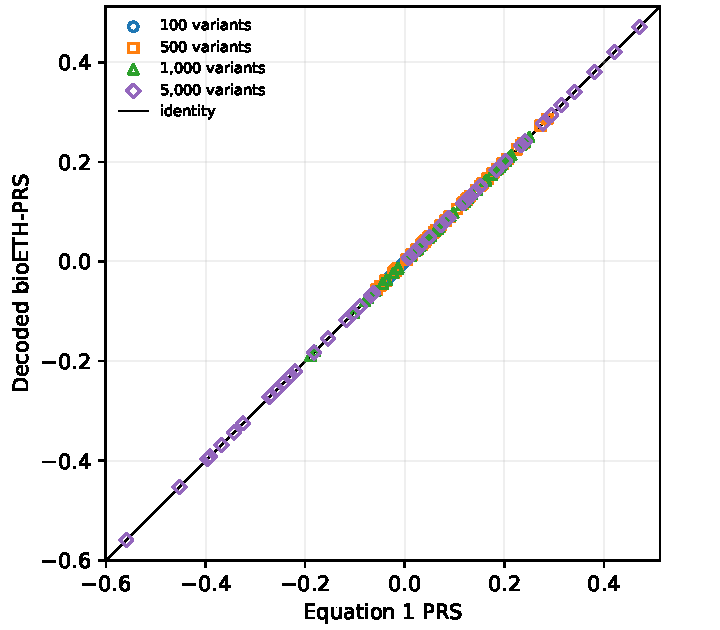
\includegraphics[width=\columnwidth, keepaspectratio]{figures/fig_individual_agreement.pdf}
  \caption{Equation~\ref{eq:prs} PRS versus decoded bioETH-PRS for all 200
  individual--fixture pairs (Hardhat mock).  Every point lies exactly on the identity
  line; overplotting is reduced by fixture-specific markers.}
  \label{fig:individual_agreement}
\end{figure}

For randomized categorical release at the 100-SNP size, agreement is 48/48 for
individuals outside the $B$-wide ambiguous band.  Two individuals lie inside the band;
both happened to agree in this run, a favorable noise draw rather than a guarantee.
Classification consumes one encoded score and is independent of variant count, so this
experiment was not repeated as a scale claim.

\subsection{Bounded Scale Evidence}

Table~\ref{tab:scale_evidence} reports fresh-model, one-sample workflow transaction
geometry.  Only the public 100-variant row is Live fhEVM.  The 100--5,000 range is
Hardhat mock, and larger rows are arithmetic projections with no execution, latency,
gas, HCU, or fee evidence.

\begin{table}[ht]
\centering
\caption{Evidence-class scale boundary.  Private mock/projection workflows add two
reader-authorization transactions; only the private 100-variant point was executed
(17 transactions, Hardhat mock).}
\label{tab:scale_evidence}
\small
\begin{tabular}{lrrr}
\toprule
\textbf{Evidence class} & \textbf{Variants} & \textbf{Visibility} & \textbf{Tx} \\
\midrule
Live fhEVM & 100 & public & 25 \\
Hardhat mock & 100 & public & 15 \\
Hardhat mock & 500 & public & 47 \\
Hardhat mock & 1,000 & public & 88 \\
Hardhat mock & 5,000 & public & 413 \\
Analytic projection & 10,000 & public & 819 \\
Analytic projection & 100,000 & public & 8,132 \\
Analytic projection & 1,000,000 & public & 81,257 \\
\bottomrule
\end{tabular}
\end{table}

\subsection{Gas Consumption and Scaling}

Figure~\ref{fig:gas} and Table~\ref{tab:gas} report total gas consumption across
execution paths and fixture sizes in the Hardhat-mock environment.  Host-contract gas
grows approximately linearly over the measured 100--5,000-variant range; this is not a
claim about live TFHE scaling.  The streaming path saves approximately 37\% above 500
variants, driven by eliminating persistent per-SNP handle storage.

\begin{figure}[t]
  \centering
  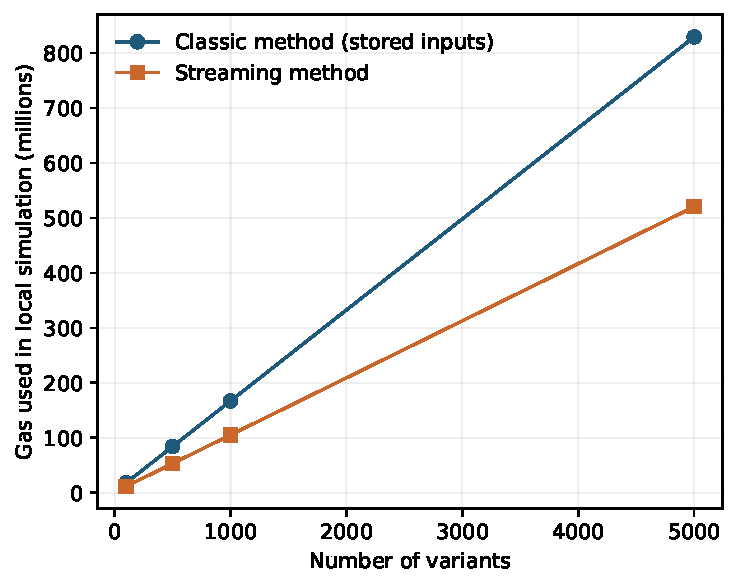
\includegraphics[width=\columnwidth, keepaspectratio]{figures/fig_gas_scaling.pdf}
  \caption{Hardhat-mock host gas versus nominal variant count for both execution
  paths.  The observed range is close to linear; no live-network scaling is inferred.
  The streaming path achieves 35.4--37.2\% lower gas by eliminating persistent
  per-SNP ciphertext-handle storage.}
  \label{fig:gas}
\end{figure}

\begin{table}[ht]
\centering
\caption{Hardhat-mock total host gas by execution path, rounded to 0.001 million gas}
\label{tab:gas}
\small
\begin{tabular}{rrrr}
\toprule
\textbf{SNPs} & \textbf{Classic} & \textbf{Streaming} & \textbf{Reduction} \\
\midrule
100   & 17.863 M & 11.538 M & 35.4\% \\
500   & 83.985 M & 53.063 M & 36.8\% \\
1,000 & 166.875 M & 105.013 M & 37.1\% \\
5,000 & 829.422 M & 520.487 M & 37.2\% \\
\bottomrule
\end{tabular}
\end{table}

\subsection{Per-SNP Cost Decomposition}

Table~\ref{tab:persnp} decomposes per-SNP gas.  The irreducible floor of
$\approx$95,000--104,000 gas/SNP comprises the input-proof verification, FHE
multiply, and FHE accumulate---operations set by the fhEVM protocol and not
reducible by contract design choices.  Future improvements in coprocessor
throughput or lighter-weight proof schemes would directly reduce this floor.

\begin{table}[ht]
\centering
\caption{Per-SNP gas decomposition}
\label{tab:persnp}
\small
\setlength{\tabcolsep}{4pt}
\begin{tabularx}{\columnwidth}{@{}Yrr@{}}
\toprule
\textbf{Operation} & \textbf{Classic} & \textbf{Streaming} \\
\midrule
Input proof verification         & $\sim$50,000 & $\sim$50,000 \\
FHE multiply                     & $\sim$27,000 & $\sim$27,000 \\
FHE accumulate (partial sum)     & $\sim$27,000 & $\sim$27,000 \\
Handle SSTORE (classic only)     &  $\sim$25,000 & --- \\
ACL SSTORE (classic only)        &  $\sim$25,000 & --- \\
SLOAD, misc.\ overhead           &   $\sim$12,000 & --- \\
\midrule
\textbf{Total/SNP}               & $\approx$\textbf{166,000} & $\approx$\textbf{104,000} \\
\bottomrule
\end{tabularx}
\end{table}

\subsection{Latency}

Hardhat-mock per-individual wall-clock measurements are 157, 780, 1,672, and
8,819 ms for 101, 501, 1,001, and 5,001 encoded positions, respectively, or
1.554--1.763 ms per position.  The roughly 13\% increase in per-position cost is
mildly superlinear over this range.  These timings combine in-process plaintext mock
arithmetic and transaction overhead; they measure neither TFHE evaluation nor network
latency.  The separate live 100-SNP timings appear in Table~\ref{tab:live_validation}
and are not compared as a speed ratio.

\subsection{Measured Transaction Use and Fee Sensitivity}

Table~\ref{tab:cost} separates observed transaction use from fee arithmetic.  The
successful live deployment used four transactions and 5.892559 million gas, costing
0.0062781714 Sepolia test ETH; the live public job used 25 transactions and 20.710271
million gas, costing 0.0252747648 test ETH.  These are test-network expenditures, not
production prices.  In the Hardhat mock, a public 100-variant streaming workflow used
15 transactions and 11.690 million gas, whereas its private counterpart required 17
transactions and 23.508 million gas (2.01$\times$).  The private configuration is the
one relevant to model-extraction risk.  Decryption is off-chain from the host contract
and adds no Ethereum transaction.

\begin{table}[ht]
\centering
\caption{Measured transaction use.  Raw evidence retains exact observations; mock
totals are rounded because encrypted calldata varies across otherwise identical runs.}
\label{tab:cost}
\footnotesize
\setlength{\tabcolsep}{2pt}
\begin{tabularx}{\columnwidth}{@{}lXrr@{}}
\toprule
\textbf{Evidence class} & \textbf{Quantity} & \textbf{Tx} & \textbf{Gas} \\
\midrule
Live fhEVM & four-contract deployment & 4 & 5.892559 M \\
Live fhEVM & public 100-SNP classic job & 25 & 20.710271 M \\
Hardhat mock & public 100-SNP streaming job & 15 & 11.690 M \\
Hardhat mock & private 100-SNP streaming job & 17 & 23.508 M \\
Hardhat mock & one-time release policy & 1 & 0.077 M \\
\bottomrule
\end{tabularx}
\end{table}

Recording nonzero model and sample provenance hashes adds a fixed 40,568 mock gas per
model; it adds no homomorphic work and does not change the HCU ceiling.  A randomized
release policy is one additional model-setup transaction (77,314 mock gas).  Raw-score
finalization (169,898 mock gas) and randomized-category finalization (432,230 mock gas)
are alternative output paths and are never summed for one job.

For sensitivity only, multiplying the mock observations by hypothetical gas prices is
an \emph{Analytic projection / unexecuted}.  At 1 gwei, the arithmetic gives 0.005892613
ETH for deployment, 0.011690021 ETH for the public job, and 0.02350788 ETH for the
private job; at 30 gwei the respective values are 0.17677839, 0.35070063, and 0.7052364
ETH.  No USD conversion, production-affordability claim, or clinical/commercial
feasibility conclusion is drawn.

\subsection{Correctness and Protocol Verification}

The independent comparison in Figure~\ref{fig:individual_agreement} verifies agreement
with Equation~\ref{eq:prs}; it is one part of a bounded correctness case rather than a
universal guarantee.  Table~\ref{tab:correctness_boundary} identifies responsibility at
each boundary.

\begin{table*}[t]
\centering
\caption{Correctness-guarantee boundary.}
\label{tab:correctness_boundary}
\small
\begin{tabularx}{\textwidth}{@{}p{3.2cm}XX@{}}
\toprule
\textbf{Actor/component} & \textbf{What is established} & \textbf{What is not established} \\
\midrule
Genotype preprocessor & build, variant order, hard-call validity, missingness policy, and effect-allele alignment & authenticity of the biological sample without attestation/binding \\
Model provider & committed weights, metadata, and fixed release policy & scientific validity, calibration, or ancestry portability \\
Smart contracts & deterministic encoded weighted sum and state/ACL policy for submitted handles & correctness of input claims or external infrastructure \\
fhEVM infrastructure & encrypted operations and authorized decryption under its assumptions & independently verified TFHE execution by consensus \\
Independent reference & exact agreement with Equation~\ref{eq:prs} on 200 fixture jobs & a proof for untested models or deployments \\
End user & can verify manifests, addresses, bytecode digests, transactions, and reference digest & clinical interpretation beyond the published model \\
\bottomrule
\end{tabularx}
\end{table*}

Protocol invariants---ACL enforcement, state-machine integrity, single finalization,
fixed model-defined thresholds, minimum threshold gap, oracle-required release,
rate-limit windows, and ACL revocation handling---are covered by the automated suite.
The protocol guarantees none of sample authenticity, clinical validity, calibration,
or ancestry portability.

%% ============================================================
\section{Access Control and Compute Flows}
\label{sec:acl}

\subsection{Encrypted Handle Lifecycle}

Every encrypted value in the fhEVM has an associated ACL record maintained in a
dedicated on-chain contract.  The ACL maps handles to authorised addresses and
distinguishes four grant types with different persistence semantics:

\begin{itemize}
  \item \textbf{Persistent contract grant}: Written to the ACL contract's persistent
        storage via SSTORE.  Allows the owning contract to use the handle in future
        transactions.  This is the primary source of gas cost in the classic upload
        path ($\approx$25,000 gas per SNP handle).
  \item \textbf{Persistent user grant}: Written to the ACL contract via SSTORE.
        Allows an end-user to decrypt the handle via the KMS gateway.  Applied at
        finalization to grant the requester access to their encoded score.
  \item \textbf{Transient grant}: Uses EIP-1153 transient storage.  Valid only for
        the current transaction.  The streaming path relies exclusively on transient
        grants for intermediate SNP handles, avoiding the SSTORE cost entirely.
  \item \textbf{Public grant}: Enables anyone to decrypt.  Applied only to the
        ternary risk category after noise addition; never applied to score values.
\end{itemize}

The ACL design is the root of the 37\% gas differential between the classic and
streaming paths.  In the classic path, each of the $N$ SNP handles requires a
persistent contract grant (SSTORE in the ACL) and a handle write to contract
storage (second SSTORE).  In the streaming path, transient grants are used for
SNP handles and the SSTORE costs are eliminated.

\subsection{State Machine and Mutual Exclusion}

The PRS Compute Engine enforces a strict job state machine to prevent incorrect
ordering of operations:
\begin{equation*}
\texttt{PENDING} \!\to\! \texttt{UPLOADING}
\!\to\! \texttt{READY}
\!\to\! \texttt{COMPUTING} \!\to\! \texttt{DONE}.
\end{equation*}
The classic and streaming paths are mutually exclusive per job.  The guard condition
uses upload counts: if any SNP handles have been written to persistent storage, the
classic path is in use and streaming calls are rejected; if computation has advanced
without persistent uploads, the streaming path is in use.  This prevents hybrid
calls that could compromise the handle-lifecycle invariants.

\subsection{Private Model Access Control}

When a GWAS model is published with private (encrypted) weights, access control is
layered: the model owner must first authorise the compute engine as a reader; individual
requesters must also be added to the private model reader list; and each compute chunk
re-checks reader authorisation, so revocation of a requester mid-job causes the next
compute chunk to fail, effectively terminating the job.  This is in contrast to the
registry ACL, which is checked only at job creation.  The asymmetric behaviour between
registry and model ACL is documented and empirically verified.

%% ============================================================
\section{Discussion}
\label{sec:discussion}

bioETH-PRS is a bounded-size research prototype for curated additive PRS models.  It
replaces the designated application-level evaluator with publicly auditable contract
orchestration while retaining explicit trust in contracts, consensus, the fhEVM
coprocessor, the relayer, and ACL/Gateway/KMS infrastructure.  The public 100-SNP path
was validated on live fhEVM; the wider 100--5,000 range and private weights were
Hardhat-mock validated.  The study therefore establishes neither a practical
genome-wide PRS engine nor clinical deployment feasibility.

\subsection{HEPRS and bioETH-PRS: Complementary Systems}

bioETH-PRS and HEPRS \citep{knight2026heprs} are best understood as complementary
rather than competing systems occupying different points in a design space defined
by trust requirements and scalability.

HEPRS demonstrates substantially larger encrypted PRS execution and real-FHE latency
under a three-party non-collusion model.  CKKS natively represents approximate signed
reals and avoids the fixed-point transformation used here.  It is the stronger evidence
base when large variant counts and measured FHE performance are the primary questions.

bioETH-PRS instead studies whether the application-level evaluator can be replaced by
an auditable policy/state-machine layer when the fhEVM and decryption infrastructure are
acceptable alternative trust anchors.  It adds on-chain model immutability, requester
authorization, fixed output policy, and a transaction audit trail, but exposes public
metadata and incurs many host-chain transactions.  These are different trust,
deployment, and performance trade-offs; neither system is broadly superior.

\subsection{Limitations and Open Problems}

\textbf{SNP count ceiling.}
The finely measured Hardhat-mock HCU ceiling is 21 SNPs for both model visibilities;
the live ceiling remains unknown.  A fresh public 5,000-variant mock workflow required
413 host transactions.  The larger rows in Table~\ref{tab:scale_evidence} are unexecuted
geometry only and show that the current architecture becomes transaction-bound well
before genome-wide scale.  No current production-cost or feasibility claim is made.

\textbf{SNP provenance.}
As specified in Section~\ref{sec:security}, ACL authorization does not bind uploaded
ciphertexts to a registered sample.  This is an explicit threat-model boundary rather
than a post hoc implementation limitation.

\textbf{URI observability.}
Sample data URIs are on-chain plaintext.  Any network node can observe storage
slots directly, even if read access is ACL-gated at the application layer.  Storing
only a cryptographic commitment to the URI would address this residual exposure.

\textbf{One-sided randomization and bias.}
Uniform noise on $[0,B)$ introduces expected upward bias and an ambiguous band around
every adjusted threshold.  The mechanism is a bounded randomized categorical release,
not differential privacy; its one-sided support, absent sensitivity calibration, and
absent composition analysis delimit the claim.

\textbf{Production cost.}
Only host gas, Sepolia test-ETH expenditure, and hypothetical ETH fee sensitivity are
reported.  Production fee schedules, USD cost, memory use, and operational throughput
were not measured, so affordability and clinical or commercial deployment practicality
remain unknown.

\subsection{Future Directions}

Planned extensions include: (1) LD-aware weighting in the encrypted domain,
incorporating LDpred2-style shrinkage \citep{prive2020ldpred2}; (2) multi-party key
generation enabling federated cohort analyses without a single decryption authority;
(3) model versioning and deprecation mechanisms; (4) SNP handle re-use across
multiple models from the same registered sample; and (5) token-based fee mechanisms
to economically incentivise model quality.  Input authenticity requires a separate
line of work: signed laboratory attestations and zero-knowledge proofs binding uploaded
ciphertexts to a committed sample and preparation manifest.  A formal privacy mechanism
would likewise require an adjacency definition, score sensitivity analysis, calibrated
noise, and composition accounting.  The current public-model multiplication converts
plaintext values to encrypted handles; a future scalar overload would reduce mock HCU
use by 38.8\%, with an estimated ceiling near 34 and approximately 148 rather than 239
compute transactions at 5,000 variants.  This optimization is not implemented or live
validated.  The architecture's modularity---four
independently upgradeable contracts---is designed to accommodate these extensions
without disrupting existing deployments.

%% ============================================================
\section{Related Work}
\label{sec:related}

Privacy-preserving genomic computation has been pursued through multiple
cryptographic paradigms.  Kim and Lauter \citep{kim2015} applied homomorphic
encryption schemes to compute GWAS statistics for up to 5,000 sequences, but did not
extend to PRS computation.  Blatt et al.\ \citep{blatt2020} built a CKKS-based
privacy-preserving GWAS pipeline for large-scale studies, noting that PRS
computation from decrypted summary statistics was future work.  McLaren et al.\
\citep{mclaren2016} demonstrated privacy-preserving genomic testing in an HIV
clinical-care model using homomorphic encryption, but did not address the full PRS
pipeline.  Raisaro et al.\ \citep{raisaro2019} introduced MedCo for secure,
privacy-preserving exploration of distributed clinical and genomic data.

Knight et al.\ \citep{knight2026heprs} (HEPRS) is the closest prior work, providing
the first complete FHE pipeline for PRS with real clinical data.  HEPRS achieves
$r > 0.999$ correlation with plaintext scores on a 110,000-SNP schizophrenia
model and demonstrates practical feasibility on commodity hardware.  bioETH-PRS
builds directly on the HEPRS computational framework and uses the same GWAS fixture
datasets, studying a different trade-off in which an auditable contract orchestrator
replaces the designated application-level evaluator while infrastructure trust remains.

On the blockchain side, prior work on privacy-preserving smart contracts has
focused on anonymous payments and related protocol work
\citep{sasson2014zerocash,pertsev2019tornado} and
zero-knowledge proof-based computation \citep{ben2018starkware}, which enable
verifiable computation but not confidential computation; ZK-SNARKs prove knowledge
without concealing the program inputs.  FHE on the blockchain, typified by the fhEVM
framework \citep{zamafhevm}, combines confidential operations with publicly auditable
contract orchestration under explicit coprocessor assumptions.  To our knowledge, bioETH-PRS is the first application of fhEVM
to clinical genomics.

%% ============================================================
\section{Conclusion}
\label{sec:conclusion}

We presented bioETH-PRS, a protocol for confidential polygenic risk
scoring using TFHE-based fully homomorphic encryption on a programmable blockchain.
Publicly auditable smart contracts replace the designated application-level evaluator
of HEPRS \citep{knight2026heprs}.  This is evaluator minimization, not removal of trust:
the protocol remains conditional on genotype preparation, model validity, contract
correctness, consensus, the fhEVM coprocessor, the relayer, and ACL/Gateway/KMS
threshold decryption.

The revised evidence establishes one public 100-SNP Live-fhEVM workflow with an exact
independent reference match.  Private weights and the wider 100--5,000-variant range are
Hardhat-mock validated only.  Across 200 mock jobs, decoded scores match Equation~\ref{eq:prs}
exactly because the fixture weights are losslessly quantised; this validates the
pipeline on those inputs rather than proving universal arithmetic accuracy.  Streaming
execution lowers mock host gas by 35.4--37.2\%, while measured adversarial results show
that fixed thresholds and rate limits reduce resolution and raise query cost without
providing differential privacy, Sybil resistance, or formal model confidentiality.

bioETH-PRS should therefore be read as a bounded-size research prototype for curated
additive PRS models and as an investigation of auditable fhEVM orchestration.  It is not
a practical genome-wide PRS engine, and the study does not establish production
affordability, clinical deployment feasibility, private-weight live execution, or a
live HCU ceiling.  HEPRS demonstrates larger encrypted execution; bioETH-PRS contributes
a smaller-scale contract policy and auditability design.  Future progress requires
measured production infrastructure, ciphertext-to-sample binding, calibrated privacy
mechanisms, and fewer host-chain transactions.

%% ============================================================
\section*{Biographical Note}
Kimon Antonios Provatas, Christos Galanopoulos, and Ilias Georgakopoulos-Soares are researchers at The University of Texas at Austin studying pharmacology, genomics, and privacy-preserving biomedical computation at the Dell Pediatric Research Institute.

%% ============================================================
\section*{Data Availability Statement}
No new datasets were generated or analysed in this study.

%% ============================================================
\section*{Code Availability Statement}
All relevant code and results can be found on GitHub at \url{https://github.com/Georgakopoulos-Soares-lab/bioETH-PRS}.

%% ============================================================
\bibliographystyle{abbrvnat}
\bibliography{bioeth_prs}

\end{document}
